\documentclass[1p]{elsarticle_modified}
%\bibliographystyle{elsarticle-num}

%\usepackage[colorlinks]{hyperref}
%\usepackage{abbrmath_seonhwa} %\Abb, \Ascr, \Acal ,\Abf, \Afrak
\usepackage{amsfonts}
\usepackage{amssymb}
\usepackage{amsmath}
\usepackage{amsthm}
\usepackage{scalefnt}
\usepackage{amsbsy}
\usepackage{kotex}
\usepackage{caption}
\usepackage{subfig}
\usepackage{color}
\usepackage{graphicx}
\usepackage{xcolor} %% white, black, red, green, blue, cyan, magenta, yellow
\usepackage{float}
\usepackage{setspace}
\usepackage{hyperref}

\usepackage{tikz}
\usetikzlibrary{arrows}

\usepackage{multirow}
\usepackage{array} % fixed length table
\usepackage{hhline}

%%%%%%%%%%%%%%%%%%%%%
\makeatletter
\renewcommand*\env@matrix[1][\arraystretch]{%
	\edef\arraystretch{#1}%
	\hskip -\arraycolsep
	\let\@ifnextchar\new@ifnextchar
	\array{*\c@MaxMatrixCols c}}
\makeatother %https://tex.stackexchange.com/questions/14071/how-can-i-increase-the-line-spacing-in-a-matrix
%%%%%%%%%%%%%%%

\usepackage[normalem]{ulem}

\newcommand{\msout}[1]{\ifmmode\text{\sout{\ensuremath{#1}}}\else\sout{#1}\fi}
%SOURCE: \msout is \stkout macro in https://tex.stackexchange.com/questions/20609/strikeout-in-math-mode

\newcommand{\cancel}[1]{
	\ifmmode
	{\color{red}\msout{#1}}
	\else
	{\color{red}\sout{#1}}
	\fi
}

\newcommand{\add}[1]{
	{\color{blue}\uwave{#1}}
}

\newcommand{\replace}[2]{
	\ifmmode
	{\color{red}\msout{#1}}{\color{blue}\uwave{#2}}
	\else
	{\color{red}\sout{#1}}{\color{blue}\uwave{#2}}
	\fi
}

\newcommand{\Sol}{\mathcal{S}} %segment
\newcommand{\D}{D} %diagram
\newcommand{\A}{\mathcal{A}} %arc


%%%%%%%%%%%%%%%%%%%%%%%%%%%%%5 test

\def\sl{\operatorname{\textup{SL}}(2,\Cbb)}
\def\psl{\operatorname{\textup{PSL}}(2,\Cbb)}
\def\quan{\mkern 1mu \triangleright \mkern 1mu}

\theoremstyle{definition}
\newtheorem{thm}{Theorem}[section]
\newtheorem{prop}[thm]{Proposition}
\newtheorem{lem}[thm]{Lemma}
\newtheorem{ques}[thm]{Question}
\newtheorem{cor}[thm]{Corollary}
\newtheorem{defn}[thm]{Definition}
\newtheorem{exam}[thm]{Example}
\newtheorem{rmk}[thm]{Remark}
\newtheorem{alg}[thm]{Algorithm}

\newcommand{\I}{\sqrt{-1}}
\begin{document}

%\begin{frontmatter}
%
%\title{Boundary parabolic representations of knots up to 8 crossings}
%
%%% Group authors per affiliation:
%\author{Yunhi Cho} 
%\address{Department of Mathematics, University of Seoul, Seoul, Korea}
%\ead{yhcho@uos.ac.kr}
%
%
%\author{Seonhwa Kim} %\fnref{s_kim}}
%\address{Center for Geometry and Physics, Institute for Basic Science, Pohang, 37673, Korea}
%\ead{ryeona17@ibs.re.kr}
%
%\author{Hyuk Kim}
%\address{Department of Mathematical Sciences, Seoul National University, Seoul 08826, Korea}
%\ead{hyukkim@snu.ac.kr}
%
%\author{Seokbeom Yoon}
%\address{Department of Mathematical Sciences, Seoul National University, Seoul, 08826,  Korea}
%\ead{sbyoon15@snu.ac.kr}
%
%\begin{abstract}
%We find all boundary parabolic representation of knots up to 8 crossings.
%
%\end{abstract}
%\begin{keyword}
%    \MSC[2010] 57M25 
%\end{keyword}
%
%\end{frontmatter}

%\linenumbers
%\tableofcontents
%
\newcommand\colored[1]{\textcolor{white}{\rule[-0.35ex]{0.8em}{1.4ex}}\kern-0.8em\color{red} #1}%
%\newcommand\colored[1]{\textcolor{white}{ #1}\kern-2.17ex	\textcolor{white}{ #1}\kern-1.81ex	\textcolor{white}{ #1}\kern-2.15ex\color{red}#1	}

{\Large $\underline{12n_{0663}~(K12n_{0663})}$}

\setlength{\tabcolsep}{10pt}
\renewcommand{\arraystretch}{1.6}
\vspace{1cm}\begin{tabular}{m{100pt}>{\centering\arraybackslash}m{274pt}}
\multirow{5}{120pt}{
	\centering
	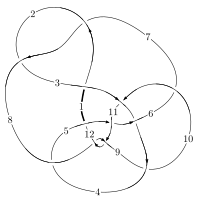
\includegraphics[width=112pt]{../../../GIT/diagram.site/Diagrams/png/2752_12n_0663.png}\\
\ \ \ A knot diagram\footnotemark}&
\allowdisplaybreaks
\textbf{Linearized knot diagam} \\
\cline{2-2}
 &
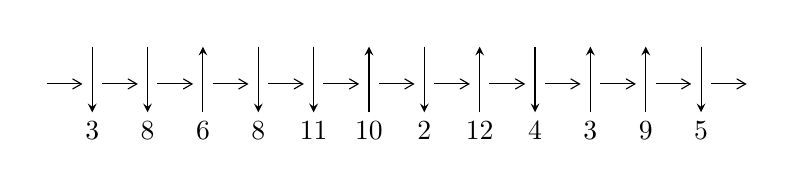
\begin{tikzpicture}[x=20pt, y=17pt]
	% nodes
	\node (C0) at (0, 0) {};
	\node (C1) at (1, 0) {};
	\node (C1U) at (1, +1) {};
	\node (C1D) at (1, -1) {3};

	\node (C2) at (2, 0) {};
	\node (C2U) at (2, +1) {};
	\node (C2D) at (2, -1) {8};

	\node (C3) at (3, 0) {};
	\node (C3U) at (3, +1) {};
	\node (C3D) at (3, -1) {6};

	\node (C4) at (4, 0) {};
	\node (C4U) at (4, +1) {};
	\node (C4D) at (4, -1) {8};

	\node (C5) at (5, 0) {};
	\node (C5U) at (5, +1) {};
	\node (C5D) at (5, -1) {11};

	\node (C6) at (6, 0) {};
	\node (C6U) at (6, +1) {};
	\node (C6D) at (6, -1) {10};

	\node (C7) at (7, 0) {};
	\node (C7U) at (7, +1) {};
	\node (C7D) at (7, -1) {2};

	\node (C8) at (8, 0) {};
	\node (C8U) at (8, +1) {};
	\node (C8D) at (8, -1) {12};

	\node (C9) at (9, 0) {};
	\node (C9U) at (9, +1) {};
	\node (C9D) at (9, -1) {4};

	\node (C10) at (10, 0) {};
	\node (C10U) at (10, +1) {};
	\node (C10D) at (10, -1) {3};

	\node (C11) at (11, 0) {};
	\node (C11U) at (11, +1) {};
	\node (C11D) at (11, -1) {9};

	\node (C12) at (12, 0) {};
	\node (C12U) at (12, +1) {};
	\node (C12D) at (12, -1) {5};
	\node (C13) at (13, 0) {};

	% arrows
	\draw[->,>={angle 60}]
	(C0) edge (C1) (C1) edge (C2) (C2) edge (C3) (C3) edge (C4) (C4) edge (C5) (C5) edge (C6) (C6) edge (C7) (C7) edge (C8) (C8) edge (C9) (C9) edge (C10) (C10) edge (C11) (C11) edge (C12) (C12) edge (C13) ;	\draw[->,>=stealth]
	(C1U) edge (C1D) (C2U) edge (C2D) (C3D) edge (C3U) (C4U) edge (C4D) (C5U) edge (C5D) (C6D) edge (C6U) (C7U) edge (C7D) (C8D) edge (C8U) (C9U) edge (C9D) (C10D) edge (C10U) (C11D) edge (C11U) (C12U) edge (C12D) ;
	\end{tikzpicture} \\
\hhline{~~} \\& 
\textbf{Solving Sequence} \\ \cline{2-2} 
 &
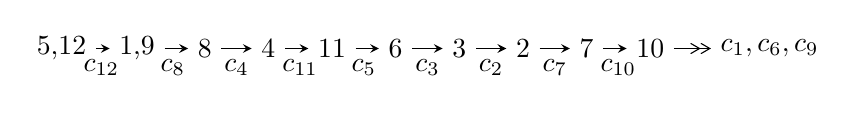
\begin{tikzpicture}[x=23pt, y=7pt]
	% node
	\node (A0) at (-1/8, 0) {5,12};
	\node (A1) at (17/16, 0) {1,9};
	\node (A2) at (17/8, 0) {8};
	\node (A3) at (25/8, 0) {4};
	\node (A4) at (33/8, 0) {11};
	\node (A5) at (41/8, 0) {6};
	\node (A6) at (49/8, 0) {3};
	\node (A7) at (57/8, 0) {2};
	\node (A8) at (65/8, 0) {7};
	\node (A9) at (73/8, 0) {10};
	\node (C1) at (1/2, -1) {$c_{12}$};
	\node (C2) at (13/8, -1) {$c_{8}$};
	\node (C3) at (21/8, -1) {$c_{4}$};
	\node (C4) at (29/8, -1) {$c_{11}$};
	\node (C5) at (37/8, -1) {$c_{5}$};
	\node (C6) at (45/8, -1) {$c_{3}$};
	\node (C7) at (53/8, -1) {$c_{2}$};
	\node (C8) at (61/8, -1) {$c_{7}$};
	\node (C9) at (69/8, -1) {$c_{10}$};
	\node (A10) at (11, 0) {$c_{1},c_{6},c_{9}$};

	% edge
	\draw[->,>=stealth]	
	(A0) edge (A1) (A1) edge (A2) (A2) edge (A3) (A3) edge (A4) (A4) edge (A5) (A5) edge (A6) (A6) edge (A7) (A7) edge (A8) (A8) edge (A9) ;
	\draw[->>,>={angle 60}]	
	(A9) edge (A10);
\end{tikzpicture} \\ 

\end{tabular} \\

\footnotetext{
The image of knot diagram is generated by the software ``\textbf{Draw programme}" developed by Andrew Bartholomew(\url{http://www.layer8.co.uk/maths/draw/index.htm\#Running-draw}), where we modified some parts for our purpose(\url{https://github.com/CATsTAILs/LinksPainter}).
}\phantom \\ \newline 
\centering \textbf{Ideals for irreducible components\footnotemark of $X_{\text{par}}$} 
 
\begin{align*}
I^u_{1}&=\langle 
-8.19807\times10^{112} u^{43}-4.22174\times10^{112} u^{42}+\cdots+2.66093\times10^{114} b-1.56181\times10^{114},\\
\phantom{I^u_{1}}&\phantom{= \langle  }-8.19807\times10^{112} u^{43}-4.22174\times10^{112} u^{42}+\cdots+2.66093\times10^{114} a-4.22274\times10^{114},\\
\phantom{I^u_{1}}&\phantom{= \langle  }u^{44}-18 u^{42}+\cdots+2 u+1\rangle \\
I^u_{2}&=\langle 
-4.22056\times10^{31} u^{30}+2.20340\times10^{32} u^{29}+\cdots+1.00720\times10^{32} b+8.09762\times10^{32},\\
\phantom{I^u_{2}}&\phantom{= \langle  }-4.22056\times10^{31} u^{30}+2.20340\times10^{32} u^{29}+\cdots+1.00720\times10^{32} a+9.10482\times10^{32},\;u^{31}+8 u^{29}+\cdots-3 u+1\rangle \\
I^u_{3}&=\langle 
5.43266\times10^{151} u^{43}-8.90811\times10^{150} u^{42}+\cdots+2.96118\times10^{156} b-3.66107\times10^{156},\\
\phantom{I^u_{3}}&\phantom{= \langle  }4.95705\times10^{158} u^{43}-6.16258\times10^{158} u^{42}+\cdots+2.92136\times10^{162} a-1.06601\times10^{163},\\
\phantom{I^u_{3}}&\phantom{= \langle  }u^{44}- u^{43}+\cdots-44412 u-15101\rangle \\
\\
\end{align*}
\raggedright * 3 irreducible components of $\dim_{\mathbb{C}}=0$, with total 119 representations.\\
\footnotetext{All coefficients of polynomials are rational numbers. But the coefficients are sometimes approximated in decimal forms when there is not enough margin.}
\newpage
\renewcommand{\arraystretch}{1}
\centering \section*{I. $I^u_{1}= \langle -8.20\times10^{112} u^{43}-4.22\times10^{112} u^{42}+\cdots+2.66\times10^{114} b-1.56\times10^{114},\;-8.20\times10^{112} u^{43}-4.22\times10^{112} u^{42}+\cdots+2.66\times10^{114} a-4.22\times10^{114},\;u^{44}-18 u^{42}+\cdots+2 u+1 \rangle$}
\flushleft \textbf{(i) Arc colorings}\\
\begin{tabular}{m{7pt} m{180pt} m{7pt} m{180pt} }
\flushright $a_{5}=$&$\begin{pmatrix}0\\u\end{pmatrix}$ \\
\flushright $a_{12}=$&$\begin{pmatrix}1\\0\end{pmatrix}$ \\
\flushright $a_{1}=$&$\begin{pmatrix}1\\u^2\end{pmatrix}$ \\
\flushright $a_{9}=$&$\begin{pmatrix}0.0308091 u^{43}+0.0158657 u^{42}+\cdots-3.90450 u+1.58694\\0.0308091 u^{43}+0.0158657 u^{42}+\cdots-3.90450 u+0.586943\end{pmatrix}$ \\
\flushright $a_{8}=$&$\begin{pmatrix}1\\0.0308091 u^{43}+0.0158657 u^{42}+\cdots-3.90450 u+0.586943\end{pmatrix}$ \\
\flushright $a_{4}=$&$\begin{pmatrix}u\\0.0158657 u^{43}+0.0189392 u^{42}+\cdots+1.52533 u-0.0308091\end{pmatrix}$ \\
\flushright $a_{11}=$&$\begin{pmatrix}0.0530718 u^{43}-0.0187857 u^{42}+\cdots-11.2966 u+1.08380\\0.0222628 u^{43}-0.0346514 u^{42}+\cdots-7.39214 u-0.503148\end{pmatrix}$ \\
\flushright $a_{6}=$&$\begin{pmatrix}0.357406 u^{43}+0.0114222 u^{42}+\cdots+6.14355 u+0.578976\\0.220586 u^{43}+0.0415889 u^{42}+\cdots+6.14139 u+0.390597\end{pmatrix}$ \\
\flushright $a_{3}=$&$\begin{pmatrix}0.102339 u^{43}-0.0535366 u^{42}+\cdots+6.75934 u+0.686328\\-0.0123699 u^{43}-0.00873329 u^{42}+\cdots+6.69838 u+0.626720\end{pmatrix}$ \\
\flushright $a_{2}=$&$\begin{pmatrix}0.0591298 u^{43}-0.0619282 u^{42}+\cdots+3.09120 u-0.165265\\0.0273984 u^{43}-0.0288691 u^{42}+\cdots+6.49347 u+0.00931667\end{pmatrix}$ \\
\flushright $a_{7}=$&$\begin{pmatrix}0.0896482 u^{43}-0.0548409 u^{42}+\cdots+0.0656990 u+0.113144\\0.0883392 u^{43}-0.0530903 u^{42}+\cdots-0.256176 u+0.163412\end{pmatrix}$ \\
\flushright $a_{10}=$&$\begin{pmatrix}0.0552606 u^{43}+0.0222813 u^{42}+\cdots-3.92001 u+1.60573\\0.0609758 u^{43}+0.0207299 u^{42}+\cdots-3.81924 u+0.723763\end{pmatrix}$\\&\end{tabular}
\flushleft \textbf{(ii) Obstruction class $= -1$}\\~\\
\flushleft \textbf{(iii) Cusp Shapes $= 2.04104 u^{43}+0.0210798 u^{42}+\cdots+86.9727 u-5.18413$}\\~\\
\newpage\renewcommand{\arraystretch}{1}
\flushleft \textbf{(iv) u-Polynomials at the component}\newline \\
\begin{tabular}{m{50pt}|m{274pt}}
Crossings & \hspace{64pt}u-Polynomials at each crossing \\
\hline $$\begin{aligned}c_{1}\end{aligned}$$&$\begin{aligned}
&u^{44}+35 u^{43}+\cdots+17825792 u+4194304
\end{aligned}$\\
\hline $$\begin{aligned}c_{2},c_{7}\end{aligned}$$&$\begin{aligned}
&u^{44}-23 u^{43}+\cdots-15360 u+2048
\end{aligned}$\\
\hline $$\begin{aligned}c_{3}\end{aligned}$$&$\begin{aligned}
&u^{44}+14 u^{43}+\cdots+38 u+4
\end{aligned}$\\
\hline $$\begin{aligned}c_{4},c_{12}\end{aligned}$$&$\begin{aligned}
&u^{44}-18 u^{42}+\cdots-2 u+1
\end{aligned}$\\
\hline $$\begin{aligned}c_{5},c_{9}\end{aligned}$$&$\begin{aligned}
&u^{44}-7 u^{42}+\cdots+89 u+21
\end{aligned}$\\
\hline $$\begin{aligned}c_{6},c_{10}\end{aligned}$$&$\begin{aligned}
&u^{44}- u^{43}+\cdots- u+1
\end{aligned}$\\
\hline $$\begin{aligned}c_{8},c_{11}\end{aligned}$$&$\begin{aligned}
&u^{44}+9 u^{43}+\cdots+172 u+16
\end{aligned}$\\
\hline
\end{tabular}\\~\\
\newpage\renewcommand{\arraystretch}{1}
\flushleft \textbf{(v) Riley Polynomials at the component}\newline \\
\begin{tabular}{m{50pt}|m{274pt}}
Crossings & \hspace{64pt}Riley Polynomials at each crossing \\
\hline $$\begin{aligned}c_{1}\end{aligned}$$&$\begin{aligned}
&y^{44}-51 y^{43}+\cdots+3298534883328 y+17592186044416
\end{aligned}$\\
\hline $$\begin{aligned}c_{2},c_{7}\end{aligned}$$&$\begin{aligned}
&y^{44}-35 y^{43}+\cdots-17825792 y+4194304
\end{aligned}$\\
\hline $$\begin{aligned}c_{3}\end{aligned}$$&$\begin{aligned}
&y^{44}-14 y^{43}+\cdots+612 y+16
\end{aligned}$\\
\hline $$\begin{aligned}c_{4},c_{12}\end{aligned}$$&$\begin{aligned}
&y^{44}-36 y^{43}+\cdots+28 y+1
\end{aligned}$\\
\hline $$\begin{aligned}c_{5},c_{9}\end{aligned}$$&$\begin{aligned}
&y^{44}-14 y^{43}+\cdots-9727 y+441
\end{aligned}$\\
\hline $$\begin{aligned}c_{6},c_{10}\end{aligned}$$&$\begin{aligned}
&y^{44}+31 y^{43}+\cdots+3 y+1
\end{aligned}$\\
\hline $$\begin{aligned}c_{8},c_{11}\end{aligned}$$&$\begin{aligned}
&y^{44}+25 y^{43}+\cdots+2896 y+256
\end{aligned}$\\
\hline
\end{tabular}\\~\\
\newpage\flushleft \textbf{(vi) Complex Volumes and Cusp Shapes}
$$\begin{array}{c|c|c}  
\text{Solutions to }I^u_{1}& \I (\text{vol} + \sqrt{-1}CS) & \text{Cusp shape}\\
 \hline 
\begin{aligned}
u &= \phantom{-}0.876522 + 0.528391 I \\
a &= \phantom{-}1.09112 + 0.98148 I \\
b &= \phantom{-}0.091117 + 0.981484 I\end{aligned}
 & -2.64902 + 0.33804 I & -9.24425 + 1.00857 I \\ \hline\begin{aligned}
u &= \phantom{-}0.876522 - 0.528391 I \\
a &= \phantom{-}1.09112 - 0.98148 I \\
b &= \phantom{-}0.091117 - 0.981484 I\end{aligned}
 & -2.64902 - 0.33804 I & -9.24425 - 1.00857 I \\ \hline\begin{aligned}
u &= \phantom{-}1.079670 + 0.134336 I \\
a &= \phantom{-}0.239829 + 0.233289 I \\
b &= -0.760171 + 0.233289 I\end{aligned}
 & -1.52443 - 0.21103 I & -4.97310 + 0. I\phantom{ +0.000000I} \\ \hline\begin{aligned}
u &= \phantom{-}1.079670 - 0.134336 I \\
a &= \phantom{-}0.239829 - 0.233289 I \\
b &= -0.760171 - 0.233289 I\end{aligned}
 & -1.52443 + 0.21103 I & -4.97310 + 0. I\phantom{ +0.000000I} \\ \hline\begin{aligned}
u &= -1.189010 + 0.306258 I \\
a &= \phantom{-}0.67617 - 1.33662 I \\
b &= -0.323832 - 1.336620 I\end{aligned}
 & -6.03434 - 1.69757 I & \phantom{-0.000000 } 0 \\ \hline\begin{aligned}
u &= -1.189010 - 0.306258 I \\
a &= \phantom{-}0.67617 + 1.33662 I \\
b &= -0.323832 + 1.336620 I\end{aligned}
 & -6.03434 + 1.69757 I & \phantom{-0.000000 } 0 \\ \hline\begin{aligned}
u &= -1.207620 + 0.405136 I \\
a &= -0.011672 + 0.201487 I \\
b &= -1.011670 + 0.201487 I\end{aligned}
 & -0.85999 + 6.23657 I & \phantom{-0.000000 } 0 \\ \hline\begin{aligned}
u &= -1.207620 - 0.405136 I \\
a &= -0.011672 - 0.201487 I \\
b &= -1.011670 - 0.201487 I\end{aligned}
 & -0.85999 - 6.23657 I & \phantom{-0.000000 } 0 \\ \hline\begin{aligned}
u &= \phantom{-}1.253320 + 0.360663 I \\
a &= \phantom{-}0.58221 - 1.41088 I \\
b &= -0.41779 - 1.41088 I\end{aligned}
 & -13.0195 - 6.3051 I & \phantom{-0.000000 } 0 \\ \hline\begin{aligned}
u &= \phantom{-}1.253320 - 0.360663 I \\
a &= \phantom{-}0.58221 + 1.41088 I \\
b &= -0.41779 + 1.41088 I\end{aligned}
 & -13.0195 + 6.3051 I & \phantom{-0.000000 } 0\\
 \hline 
 \end{array}$$\newpage$$\begin{array}{c|c|c}  
\text{Solutions to }I^u_{1}& \I (\text{vol} + \sqrt{-1}CS) & \text{Cusp shape}\\
 \hline 
\begin{aligned}
u &= \phantom{-}0.609637 + 0.085004 I \\
a &= \phantom{-}0.800710 + 0.311107 I \\
b &= -0.199290 + 0.311107 I\end{aligned}
 & -1.232890 - 0.407507 I & -8.23914 + 1.51919 I \\ \hline\begin{aligned}
u &= \phantom{-}0.609637 - 0.085004 I \\
a &= \phantom{-}0.800710 - 0.311107 I \\
b &= -0.199290 - 0.311107 I\end{aligned}
 & -1.232890 + 0.407507 I & -8.23914 - 1.51919 I \\ \hline\begin{aligned}
u &= -0.15451 + 1.43462 I \\
a &= \phantom{-}0.738629 - 0.751056 I \\
b &= -0.261371 - 0.751056 I\end{aligned}
 & \phantom{-}2.74125 - 1.62157 I & \phantom{-0.000000 } 0 \\ \hline\begin{aligned}
u &= -0.15451 - 1.43462 I \\
a &= \phantom{-}0.738629 + 0.751056 I \\
b &= -0.261371 + 0.751056 I\end{aligned}
 & \phantom{-}2.74125 + 1.62157 I & \phantom{-0.000000 } 0 \\ \hline\begin{aligned}
u &= -0.399143 + 0.330546 I \\
a &= \phantom{-}1.40923 - 0.92070 I \\
b &= \phantom{-}0.409229 - 0.920695 I\end{aligned}
 & \phantom{-}0.05653 - 2.19737 I & \phantom{-}0.00628 + 3.06449 I \\ \hline\begin{aligned}
u &= -0.399143 - 0.330546 I \\
a &= \phantom{-}1.40923 + 0.92070 I \\
b &= \phantom{-}0.409229 + 0.920695 I\end{aligned}
 & \phantom{-}0.05653 + 2.19737 I & \phantom{-}0.00628 - 3.06449 I \\ \hline\begin{aligned}
u &= -1.50977 + 0.31090 I \\
a &= \phantom{-}0.560340 + 1.196140 I \\
b &= -0.439660 + 1.196140 I\end{aligned}
 & -12.57110 + 0.21179 I & \phantom{-0.000000 } 0 \\ \hline\begin{aligned}
u &= -1.50977 - 0.31090 I \\
a &= \phantom{-}0.560340 - 1.196140 I \\
b &= -0.439660 - 1.196140 I\end{aligned}
 & -12.57110 - 0.21179 I & \phantom{-0.000000 } 0 \\ \hline\begin{aligned}
u &= \phantom{-}0.414615 + 0.126074 I \\
a &= \phantom{-}1.46142 + 1.21039 I \\
b &= \phantom{-}0.461422 + 1.210400 I\end{aligned}
 & -2.58939 + 6.06896 I & -6.96240 - 5.29777 I \\ \hline\begin{aligned}
u &= \phantom{-}0.414615 - 0.126074 I \\
a &= \phantom{-}1.46142 - 1.21039 I \\
b &= \phantom{-}0.461422 - 1.210400 I\end{aligned}
 & -2.58939 - 6.06896 I & -6.96240 + 5.29777 I\\
 \hline 
 \end{array}$$\newpage$$\begin{array}{c|c|c}  
\text{Solutions to }I^u_{1}& \I (\text{vol} + \sqrt{-1}CS) & \text{Cusp shape}\\
 \hline 
\begin{aligned}
u &= \phantom{-}1.54962 + 0.23074 I \\
a &= \phantom{-}0.439073 + 1.200720 I \\
b &= -0.560927 + 1.200720 I\end{aligned}
 & -4.34261 - 4.88782 I & \phantom{-0.000000 } 0 \\ \hline\begin{aligned}
u &= \phantom{-}1.54962 - 0.23074 I \\
a &= \phantom{-}0.439073 - 1.200720 I \\
b &= -0.560927 - 1.200720 I\end{aligned}
 & -4.34261 + 4.88782 I & \phantom{-0.000000 } 0 \\ \hline\begin{aligned}
u &= -1.33716 + 0.82047 I \\
a &= \phantom{-}0.163799 + 0.042605 I \\
b &= -0.836201 + 0.042605 I\end{aligned}
 & -8.84801 + 4.59946 I & \phantom{-0.000000 } 0 \\ \hline\begin{aligned}
u &= -1.33716 - 0.82047 I \\
a &= \phantom{-}0.163799 - 0.042605 I \\
b &= -0.836201 - 0.042605 I\end{aligned}
 & -8.84801 - 4.59946 I & \phantom{-0.000000 } 0 \\ \hline\begin{aligned}
u &= \phantom{-}0.53152 + 1.54489 I \\
a &= \phantom{-}0.728029 + 0.866444 I \\
b &= -0.271971 + 0.866444 I\end{aligned}
 & \phantom{-}2.40594 - 4.26197 I & \phantom{-0.000000 } 0 \\ \hline\begin{aligned}
u &= \phantom{-}0.53152 - 1.54489 I \\
a &= \phantom{-}0.728029 - 0.866444 I \\
b &= -0.271971 - 0.866444 I\end{aligned}
 & \phantom{-}2.40594 + 4.26197 I & \phantom{-0.000000 } 0 \\ \hline\begin{aligned}
u &= -0.071957 + 0.347959 I \\
a &= \phantom{-}1.68636 - 0.27524 I \\
b &= \phantom{-}0.686363 - 0.275238 I\end{aligned}
 & \phantom{-}1.56185 - 1.94947 I & \phantom{-}2.03078 + 4.77946 I \\ \hline\begin{aligned}
u &= -0.071957 - 0.347959 I \\
a &= \phantom{-}1.68636 + 0.27524 I \\
b &= \phantom{-}0.686363 + 0.275238 I\end{aligned}
 & \phantom{-}1.56185 + 1.94947 I & \phantom{-}2.03078 - 4.77946 I \\ \hline\begin{aligned}
u &= \phantom{-}1.37910 + 0.91921 I \\
a &= -0.0534857 - 0.1038620 I \\
b &= -1.053490 - 0.103862 I\end{aligned}
 & -8.1171 - 11.6018 I & \phantom{-0.000000 } 0 \\ \hline\begin{aligned}
u &= \phantom{-}1.37910 - 0.91921 I \\
a &= -0.0534857 + 0.1038620 I \\
b &= -1.053490 + 0.103862 I\end{aligned}
 & -8.1171 + 11.6018 I & \phantom{-0.000000 } 0\\
 \hline 
 \end{array}$$\newpage$$\begin{array}{c|c|c}  
\text{Solutions to }I^u_{1}& \I (\text{vol} + \sqrt{-1}CS) & \text{Cusp shape}\\
 \hline 
\begin{aligned}
u &= -1.64285 + 0.31556 I \\
a &= \phantom{-}1.00976 - 1.01253 I \\
b &= \phantom{-}0.009762 - 1.012530 I\end{aligned}
 & -10.55820 - 0.01477 I & \phantom{-0.000000 } 0 \\ \hline\begin{aligned}
u &= -1.64285 - 0.31556 I \\
a &= \phantom{-}1.00976 + 1.01253 I \\
b &= \phantom{-}0.009762 + 1.012530 I\end{aligned}
 & -10.55820 + 0.01477 I & \phantom{-0.000000 } 0 \\ \hline\begin{aligned}
u &= \phantom{-}1.44509 + 0.84306 I \\
a &= \phantom{-}0.610238 + 1.224140 I \\
b &= -0.389762 + 1.224140 I\end{aligned}
 & -5.59770 - 4.07714 I & \phantom{-0.000000 } 0 \\ \hline\begin{aligned}
u &= \phantom{-}1.44509 - 0.84306 I \\
a &= \phantom{-}0.610238 - 1.224140 I \\
b &= -0.389762 - 1.224140 I\end{aligned}
 & -5.59770 + 4.07714 I & \phantom{-0.000000 } 0 \\ \hline\begin{aligned}
u &= -1.59950 + 0.65744 I \\
a &= \phantom{-}0.417136 - 1.269310 I \\
b &= -0.582864 - 1.269310 I\end{aligned}
 & -4.18114 + 11.97330 I & \phantom{-0.000000 } 0 \\ \hline\begin{aligned}
u &= -1.59950 - 0.65744 I \\
a &= \phantom{-}0.417136 + 1.269310 I \\
b &= -0.582864 + 1.269310 I\end{aligned}
 & -4.18114 - 11.97330 I & \phantom{-0.000000 } 0 \\ \hline\begin{aligned}
u &= -0.142365 + 0.099749 I \\
a &= \phantom{-}2.04560 + 0.61037 I \\
b &= \phantom{-}1.045600 + 0.610374 I\end{aligned}
 & \phantom{-}2.62916 + 1.12288 I & -7.07882 + 9.08866 I \\ \hline\begin{aligned}
u &= -0.142365 - 0.099749 I \\
a &= \phantom{-}2.04560 - 0.61037 I \\
b &= \phantom{-}1.045600 - 0.610374 I\end{aligned}
 & \phantom{-}2.62916 - 1.12288 I & -7.07882 - 9.08866 I \\ \hline\begin{aligned}
u &= \phantom{-}0.044194 + 0.164660 I \\
a &= \phantom{-}1.93626 - 1.21271 I \\
b &= \phantom{-}0.93626 - 1.21271 I\end{aligned}
 & \phantom{-}0.80464 - 6.11087 I & -11.6087 + 22.8648 I \\ \hline\begin{aligned}
u &= \phantom{-}0.044194 - 0.164660 I \\
a &= \phantom{-}1.93626 + 1.21271 I \\
b &= \phantom{-}0.93626 + 1.21271 I\end{aligned}
 & \phantom{-}0.80464 + 6.11087 I & -11.6087 - 22.8648 I\\
 \hline 
 \end{array}$$\newpage$$\begin{array}{c|c|c}  
\text{Solutions to }I^u_{1}& \I (\text{vol} + \sqrt{-1}CS) & \text{Cusp shape}\\
 \hline 
\begin{aligned}
u &= -1.67061 + 1.16694 I \\
a &= \phantom{-}0.531277 - 1.236650 I \\
b &= -0.468723 - 1.236650 I\end{aligned}
 & -12.4436 + 9.3189 I & \phantom{-0.000000 } 0 \\ \hline\begin{aligned}
u &= -1.67061 - 1.16694 I \\
a &= \phantom{-}0.531277 + 1.236650 I \\
b &= -0.468723 + 1.236650 I\end{aligned}
 & -12.4436 - 9.3189 I & \phantom{-0.000000 } 0 \\ \hline\begin{aligned}
u &= \phantom{-}1.74121 + 1.12234 I \\
a &= \phantom{-}0.437976 + 1.307160 I \\
b &= -0.56202 + 1.30716 I\end{aligned}
 & -11.8590 - 17.3430 I & \phantom{-0.000000 } 0 \\ \hline\begin{aligned}
u &= \phantom{-}1.74121 - 1.12234 I \\
a &= \phantom{-}0.437976 - 1.307160 I \\
b &= -0.56202 - 1.30716 I\end{aligned}
 & -11.8590 + 17.3430 I & \phantom{-0.000000 } 0\\
 \hline 
 \end{array}$$\newpage\newpage\renewcommand{\arraystretch}{1}
\centering \section*{II. $I^u_{2}= \langle -4.22\times10^{31} u^{30}+2.20\times10^{32} u^{29}+\cdots+1.01\times10^{32} b+8.10\times10^{32},\;-4.22\times10^{31} u^{30}+2.20\times10^{32} u^{29}+\cdots+1.01\times10^{32} a+9.10\times10^{32},\;u^{31}+8 u^{29}+\cdots-3 u+1 \rangle$}
\flushleft \textbf{(i) Arc colorings}\\
\begin{tabular}{m{7pt} m{180pt} m{7pt} m{180pt} }
\flushright $a_{5}=$&$\begin{pmatrix}0\\u\end{pmatrix}$ \\
\flushright $a_{12}=$&$\begin{pmatrix}1\\0\end{pmatrix}$ \\
\flushright $a_{1}=$&$\begin{pmatrix}1\\u^2\end{pmatrix}$ \\
\flushright $a_{9}=$&$\begin{pmatrix}0.419039 u^{30}-2.18765 u^{29}+\cdots+14.5202 u-9.03974\\0.419039 u^{30}-2.18765 u^{29}+\cdots+14.5202 u-8.03974\end{pmatrix}$ \\
\flushright $a_{8}=$&$\begin{pmatrix}-1\\0.419039 u^{30}-2.18765 u^{29}+\cdots+14.5202 u-8.03974\end{pmatrix}$ \\
\flushright $a_{4}=$&$\begin{pmatrix}u\\2.18765 u^{30}+1.08094 u^{29}+\cdots+7.78263 u+0.419039\end{pmatrix}$ \\
\flushright $a_{11}=$&$\begin{pmatrix}-0.500932 u^{30}-1.84733 u^{29}+\cdots+5.71896 u-7.55669\\-0.0818935 u^{30}-4.03498 u^{29}+\cdots+20.2391 u-16.5964\end{pmatrix}$ \\
\flushright $a_{6}=$&$\begin{pmatrix}-0.134161 u^{30}+0.273690 u^{29}+\cdots+1.51196 u-0.199830\\1.24808 u^{30}+0.183025 u^{29}+\cdots+10.7167 u-3.11982\end{pmatrix}$ \\
\flushright $a_{3}=$&$\begin{pmatrix}1.57804 u^{30}+0.544822 u^{29}+\cdots+4.95031 u-0.596126\\2.25205 u^{30}+0.921857 u^{29}+\cdots+5.25234 u+1.41922\end{pmatrix}$ \\
\flushright $a_{2}=$&$\begin{pmatrix}2.13048 u^{30}+0.190785 u^{29}+\cdots+9.66763 u-1.11457\\-2.66458 u^{30}+1.29047 u^{29}+\cdots-27.0753 u+10.7100\end{pmatrix}$ \\
\flushright $a_{7}=$&$\begin{pmatrix}0.914126 u^{30}+0.818689 u^{29}+\cdots+0.245607 u+2.56016\\-5.70362 u^{30}-1.64130 u^{29}+\cdots-27.9449 u+3.71554\end{pmatrix}$ \\
\flushright $a_{10}=$&$\begin{pmatrix}1.18661 u^{30}-2.18060 u^{29}+\cdots+19.5612 u-10.8871\\0.509703 u^{30}-1.77620 u^{29}+\cdots+13.2934 u-6.65750\end{pmatrix}$\\&\end{tabular}
\flushleft \textbf{(ii) Obstruction class $= 1$}\\~\\
\flushleft \textbf{(iii) Cusp Shapes $= -5.23434 u^{30}-0.611283 u^{29}+\cdots+1.07019 u+13.5933$}\\~\\
\newpage\renewcommand{\arraystretch}{1}
\flushleft \textbf{(iv) u-Polynomials at the component}\newline \\
\begin{tabular}{m{50pt}|m{274pt}}
Crossings & \hspace{64pt}u-Polynomials at each crossing \\
\hline $$\begin{aligned}c_{1}\end{aligned}$$&$\begin{aligned}
&u^{31}-32 u^{30}+\cdots+18 u-1
\end{aligned}$\\
\hline $$\begin{aligned}c_{2}\end{aligned}$$&$\begin{aligned}
&u^{31}-16 u^{29}+\cdots-6 u+1
\end{aligned}$\\
\hline $$\begin{aligned}c_{3}\end{aligned}$$&$\begin{aligned}
&u^{31}+19 u^{30}+\cdots+13 u+1
\end{aligned}$\\
\hline $$\begin{aligned}c_{4},c_{12}\end{aligned}$$&$\begin{aligned}
&u^{31}+8 u^{29}+\cdots-3 u+1
\end{aligned}$\\
\hline $$\begin{aligned}c_{5},c_{9}\end{aligned}$$&$\begin{aligned}
&u^{31}- u^{29}+\cdots+7 u^2-1
\end{aligned}$\\
\hline $$\begin{aligned}c_{6},c_{10}\end{aligned}$$&$\begin{aligned}
&u^{31}- u^{30}+\cdots-9 u^3-1
\end{aligned}$\\
\hline $$\begin{aligned}c_{7}\end{aligned}$$&$\begin{aligned}
&u^{31}-16 u^{29}+\cdots-6 u-1
\end{aligned}$\\
\hline $$\begin{aligned}c_{8}\end{aligned}$$&$\begin{aligned}
&u^{31}+10 u^{30}+\cdots+11 u+5
\end{aligned}$\\
\hline $$\begin{aligned}c_{11}\end{aligned}$$&$\begin{aligned}
&u^{31}-10 u^{30}+\cdots+11 u-5
\end{aligned}$\\
\hline
\end{tabular}\\~\\
\newpage\renewcommand{\arraystretch}{1}
\flushleft \textbf{(v) Riley Polynomials at the component}\newline \\
\begin{tabular}{m{50pt}|m{274pt}}
Crossings & \hspace{64pt}Riley Polynomials at each crossing \\
\hline $$\begin{aligned}c_{1}\end{aligned}$$&$\begin{aligned}
&y^{31}-44 y^{30}+\cdots-1382 y-1
\end{aligned}$\\
\hline $$\begin{aligned}c_{2},c_{7}\end{aligned}$$&$\begin{aligned}
&y^{31}-32 y^{30}+\cdots+18 y-1
\end{aligned}$\\
\hline $$\begin{aligned}c_{3}\end{aligned}$$&$\begin{aligned}
&y^{31}-13 y^{30}+\cdots+11 y-1
\end{aligned}$\\
\hline $$\begin{aligned}c_{4},c_{12}\end{aligned}$$&$\begin{aligned}
&y^{31}+16 y^{30}+\cdots-9 y-1
\end{aligned}$\\
\hline $$\begin{aligned}c_{5},c_{9}\end{aligned}$$&$\begin{aligned}
&y^{31}-2 y^{30}+\cdots+14 y-1
\end{aligned}$\\
\hline $$\begin{aligned}c_{6},c_{10}\end{aligned}$$&$\begin{aligned}
&y^{31}-13 y^{30}+\cdots+6 y^2-1
\end{aligned}$\\
\hline $$\begin{aligned}c_{8},c_{11}\end{aligned}$$&$\begin{aligned}
&y^{31}+18 y^{30}+\cdots-169 y-25
\end{aligned}$\\
\hline
\end{tabular}\\~\\
\newpage\flushleft \textbf{(vi) Complex Volumes and Cusp Shapes}
$$\begin{array}{c|c|c}  
\text{Solutions to }I^u_{2}& \I (\text{vol} + \sqrt{-1}CS) & \text{Cusp shape}\\
 \hline 
\begin{aligned}
u &= -0.452905 + 0.853811 I \\
a &= -0.41115 + 1.40701 I \\
b &= \phantom{-}0.58885 + 1.40701 I\end{aligned}
 & -1.88667 + 7.24502 I & -3.56693 - 12.29348 I \\ \hline\begin{aligned}
u &= -0.452905 - 0.853811 I \\
a &= -0.41115 - 1.40701 I \\
b &= \phantom{-}0.58885 - 1.40701 I\end{aligned}
 & -1.88667 - 7.24502 I & -3.56693 + 12.29348 I \\ \hline\begin{aligned}
u &= -0.537908 + 0.776764 I \\
a &= -1.25638 + 0.81390 I \\
b &= -0.256377 + 0.813898 I\end{aligned}
 & \phantom{-}1.05321 - 4.42170 I & \phantom{-}1.63233 + 2.08309 I \\ \hline\begin{aligned}
u &= -0.537908 - 0.776764 I \\
a &= -1.25638 - 0.81390 I \\
b &= -0.256377 - 0.813898 I\end{aligned}
 & \phantom{-}1.05321 + 4.42170 I & \phantom{-}1.63233 - 2.08309 I \\ \hline\begin{aligned}
u &= \phantom{-}0.186959 + 0.922387 I \\
a &= \phantom{-}0.136989 + 0.093867 I \\
b &= \phantom{-}1.136990 + 0.093867 I\end{aligned}
 & \phantom{-}2.74478 + 1.10405 I & \phantom{-}4.27026 - 4.94566 I \\ \hline\begin{aligned}
u &= \phantom{-}0.186959 - 0.922387 I \\
a &= \phantom{-}0.136989 - 0.093867 I \\
b &= \phantom{-}1.136990 - 0.093867 I\end{aligned}
 & \phantom{-}2.74478 - 1.10405 I & \phantom{-}4.27026 + 4.94566 I \\ \hline\begin{aligned}
u &= \phantom{-}0.785470 + 0.888097 I \\
a &= -0.68298 - 1.26508 I \\
b &= \phantom{-}0.317017 - 1.265080 I\end{aligned}
 & -2.98382 - 5.05597 I & -1.85048 + 6.61092 I \\ \hline\begin{aligned}
u &= \phantom{-}0.785470 - 0.888097 I \\
a &= -0.68298 + 1.26508 I \\
b &= \phantom{-}0.317017 + 1.265080 I\end{aligned}
 & -2.98382 + 5.05597 I & -1.85048 - 6.61092 I \\ \hline\begin{aligned}
u &= \phantom{-}0.716103 + 0.268510 I \\
a &= -1.33254 - 1.08651 I \\
b &= -0.332542 - 1.086510 I\end{aligned}
 & -0.64391 + 6.63799 I & -4.09253 - 8.74235 I \\ \hline\begin{aligned}
u &= \phantom{-}0.716103 - 0.268510 I \\
a &= -1.33254 + 1.08651 I \\
b &= -0.332542 + 1.086510 I\end{aligned}
 & -0.64391 - 6.63799 I & -4.09253 + 8.74235 I\\
 \hline 
 \end{array}$$\newpage$$\begin{array}{c|c|c}  
\text{Solutions to }I^u_{2}& \I (\text{vol} + \sqrt{-1}CS) & \text{Cusp shape}\\
 \hline 
\begin{aligned}
u &= \phantom{-}0.870665 + 0.895756 I \\
a &= -0.413460 - 1.291070 I \\
b &= \phantom{-}0.58654 - 1.29107 I\end{aligned}
 & -0.92154 - 4.91630 I & -0.630490 + 1.059159 I \\ \hline\begin{aligned}
u &= \phantom{-}0.870665 - 0.895756 I \\
a &= -0.413460 + 1.291070 I \\
b &= \phantom{-}0.58654 + 1.29107 I\end{aligned}
 & -0.92154 + 4.91630 I & -0.630490 - 1.059159 I \\ \hline\begin{aligned}
u &= -1.28812\phantom{ +0.000000I} \\
a &= \phantom{-}0.0316573\phantom{ +0.000000I} \\
b &= \phantom{-}1.03166\phantom{ +0.000000I}\end{aligned}
 & -5.54014\phantom{ +0.000000I} & -6.97090\phantom{ +0.000000I} \\ \hline\begin{aligned}
u &= \phantom{-}0.337074 + 0.547150 I \\
a &= -1.333870 - 0.200623 I \\
b &= -0.333874 - 0.200623 I\end{aligned}
 & \phantom{-}1.82880 - 3.66778 I & \phantom{-}3.40426 + 8.66722 I \\ \hline\begin{aligned}
u &= \phantom{-}0.337074 - 0.547150 I \\
a &= -1.333870 + 0.200623 I \\
b &= -0.333874 + 0.200623 I\end{aligned}
 & \phantom{-}1.82880 + 3.66778 I & \phantom{-}3.40426 - 8.66722 I \\ \hline\begin{aligned}
u &= -0.550474 + 0.090472 I \\
a &= -1.48951 + 0.83661 I \\
b &= -0.489508 + 0.836612 I\end{aligned}
 & \phantom{-}0.747383 + 1.132650 I & -2.64987 + 1.35406 I \\ \hline\begin{aligned}
u &= -0.550474 - 0.090472 I \\
a &= -1.48951 - 0.83661 I \\
b &= -0.489508 - 0.836612 I\end{aligned}
 & \phantom{-}0.747383 - 1.132650 I & -2.64987 - 1.35406 I \\ \hline\begin{aligned}
u &= \phantom{-}0.275688 + 0.445827 I \\
a &= \phantom{-}0.090985 - 0.553978 I \\
b &= \phantom{-}1.090990 - 0.553978 I\end{aligned}
 & \phantom{-}2.79142 - 1.37520 I & \phantom{-}7.9988 + 12.6336 I \\ \hline\begin{aligned}
u &= \phantom{-}0.275688 - 0.445827 I \\
a &= \phantom{-}0.090985 + 0.553978 I \\
b &= \phantom{-}1.090990 + 0.553978 I\end{aligned}
 & \phantom{-}2.79142 + 1.37520 I & \phantom{-}7.9988 - 12.6336 I \\ \hline\begin{aligned}
u &= -0.03863 + 1.48036 I \\
a &= -0.685298 + 0.806812 I \\
b &= \phantom{-}0.314702 + 0.806812 I\end{aligned}
 & \phantom{-}2.64360 - 1.37646 I & -7.6626 - 13.0384 I\\
 \hline 
 \end{array}$$\newpage$$\begin{array}{c|c|c}  
\text{Solutions to }I^u_{2}& \I (\text{vol} + \sqrt{-1}CS) & \text{Cusp shape}\\
 \hline 
\begin{aligned}
u &= -0.03863 - 1.48036 I \\
a &= -0.685298 - 0.806812 I \\
b &= \phantom{-}0.314702 - 0.806812 I\end{aligned}
 & \phantom{-}2.64360 + 1.37646 I & -7.6626 + 13.0384 I \\ \hline\begin{aligned}
u &= \phantom{-}0.56127 + 1.43073 I \\
a &= -0.718872 - 0.806067 I \\
b &= \phantom{-}0.281128 - 0.806067 I\end{aligned}
 & \phantom{-}2.65382 - 4.19990 I & \phantom{-}12.92958 + 1.02953 I \\ \hline\begin{aligned}
u &= \phantom{-}0.56127 - 1.43073 I \\
a &= -0.718872 + 0.806067 I \\
b &= \phantom{-}0.281128 + 0.806067 I\end{aligned}
 & \phantom{-}2.65382 + 4.19990 I & \phantom{-}12.92958 - 1.02953 I \\ \hline\begin{aligned}
u &= \phantom{-}0.181284 + 0.425324 I \\
a &= -0.071576 + 1.199900 I \\
b &= \phantom{-}0.92842 + 1.19990 I\end{aligned}
 & \phantom{-}0.90637 + 5.93162 I & \phantom{-}7.27226 + 10.53139 I \\ \hline\begin{aligned}
u &= \phantom{-}0.181284 - 0.425324 I \\
a &= -0.071576 - 1.199900 I \\
b &= \phantom{-}0.92842 - 1.19990 I\end{aligned}
 & \phantom{-}0.90637 - 5.93162 I & \phantom{-}7.27226 - 10.53139 I \\ \hline\begin{aligned}
u &= -1.49593 + 0.44328 I \\
a &= -0.52089 + 1.33114 I \\
b &= \phantom{-}0.47911 + 1.33114 I\end{aligned}
 & -9.78380 + 5.35394 I & -8.97149 - 3.53143 I \\ \hline\begin{aligned}
u &= -1.49593 - 0.44328 I \\
a &= -0.52089 - 1.33114 I \\
b &= \phantom{-}0.47911 - 1.33114 I\end{aligned}
 & -9.78380 - 5.35394 I & -8.97149 + 3.53143 I \\ \hline\begin{aligned}
u &= -0.44448 + 1.60114 I \\
a &= -0.874742 + 1.099660 I \\
b &= \phantom{-}0.125258 + 1.099660 I\end{aligned}
 & -8.55901 + 4.17105 I & -9.11820 + 0. I\phantom{ +0.000000I} \\ \hline\begin{aligned}
u &= -0.44448 - 1.60114 I \\
a &= -0.874742 - 1.099660 I \\
b &= \phantom{-}0.125258 - 1.099660 I\end{aligned}
 & -8.55901 - 4.17105 I & -9.11820 + 0. I\phantom{ +0.000000I} \\ \hline\begin{aligned}
u &= \phantom{-}0.24987 + 1.74772 I \\
a &= -0.952529 - 0.868304 I \\
b &= \phantom{-}0.047471 - 0.868304 I\end{aligned}
 & -7.55978 + 3.46072 I & \phantom{-0.000000 } 0\\
 \hline 
 \end{array}$$\newpage$$\begin{array}{c|c|c}  
\text{Solutions to }I^u_{2}& \I (\text{vol} + \sqrt{-1}CS) & \text{Cusp shape}\\
 \hline 
\begin{aligned}
u &= \phantom{-}0.24987 - 1.74772 I \\
a &= -0.952529 + 0.868304 I \\
b &= \phantom{-}0.047471 + 0.868304 I\end{aligned}
 & -7.55978 - 3.46072 I & \phantom{-0.000000 } 0\\
 \hline 
 \end{array}$$\newpage\newpage\renewcommand{\arraystretch}{1}
\centering \section*{III. $I^u_{3}= \langle 5.43\times10^{151} u^{43}-8.91\times10^{150} u^{42}+\cdots+2.96\times10^{156} b-3.66\times10^{156},\;4.96\times10^{158} u^{43}-6.16\times10^{158} u^{42}+\cdots+2.92\times10^{162} a-1.07\times10^{163},\;u^{44}- u^{43}+\cdots-44412 u-15101 \rangle$}
\flushleft \textbf{(i) Arc colorings}\\
\begin{tabular}{m{7pt} m{180pt} m{7pt} m{180pt} }
\flushright $a_{5}=$&$\begin{pmatrix}0\\u\end{pmatrix}$ \\
\flushright $a_{12}=$&$\begin{pmatrix}1\\0\end{pmatrix}$ \\
\flushright $a_{1}=$&$\begin{pmatrix}1\\u^2\end{pmatrix}$ \\
\flushright $a_{9}=$&$\begin{pmatrix}-0.000169683 u^{43}+0.000210949 u^{42}+\cdots+5.78299 u+3.64903\\-0.0000183462 u^{43}+3.00829\times10^{-6} u^{42}+\cdots+0.211471 u+1.23635\end{pmatrix}$ \\
\flushright $a_{8}=$&$\begin{pmatrix}-0.000151336 u^{43}+0.000207940 u^{42}+\cdots+5.57152 u+2.41268\\-0.0000183462 u^{43}+3.00829\times10^{-6} u^{42}+\cdots+0.211471 u+1.23635\end{pmatrix}$ \\
\flushright $a_{4}=$&$\begin{pmatrix}-0.0000756392 u^{43}+0.0000596207 u^{42}+\cdots+5.24244 u+3.86675\\0.0000561723 u^{43}-0.0000698589 u^{42}+\cdots-2.23717 u-0.996626\end{pmatrix}$ \\
\flushright $a_{11}=$&$\begin{pmatrix}-0.0000850891 u^{43}+0.000117555 u^{42}+\cdots+3.71467 u+1.98036\\-0.0000190918 u^{43}-4.61504\times10^{-6} u^{42}+\cdots+1.55518 u+1.28646\end{pmatrix}$ \\
\flushright $a_{6}=$&$\begin{pmatrix}0.0000606296 u^{43}-0.0000562866 u^{42}+\cdots-1.42364 u-1.02194\\-0.0000643844 u^{43}+0.000160536 u^{42}+\cdots+2.39137 u-0.0933425\end{pmatrix}$ \\
\flushright $a_{3}=$&$\begin{pmatrix}-0.000156271 u^{43}+0.000208628 u^{42}+\cdots+5.58861 u+4.03110\\-0.0000100454 u^{43}-0.0000181491 u^{42}+\cdots-0.0516493 u+1.17222\end{pmatrix}$ \\
\flushright $a_{2}=$&$\begin{pmatrix}-0.0000549133 u^{43}+0.0000701005 u^{42}+\cdots+1.66912 u+2.45455\\2.89573\times10^{-6} u^{43}-0.0000135692 u^{42}+\cdots-0.206033 u+0.374072\end{pmatrix}$ \\
\flushright $a_{7}=$&$\begin{pmatrix}-0.000202715 u^{43}+0.000277055 u^{42}+\cdots+7.83899 u+4.15309\\-0.0000258823 u^{43}-9.15989\times10^{-6} u^{42}+\cdots+0.308767 u+1.59630\end{pmatrix}$ \\
\flushright $a_{10}=$&$\begin{pmatrix}-0.000217536 u^{43}+0.000305300 u^{42}+\cdots+9.06131 u+5.15377\\-0.0000433575 u^{43}-4.00488\times10^{-6} u^{42}+\cdots+2.70727 u+2.71279\end{pmatrix}$\\&\end{tabular}
\flushleft \textbf{(ii) Obstruction class $= -1$}\\~\\
\flushleft \textbf{(iii) Cusp Shapes $= 0.000482548 u^{43}-0.000947210 u^{42}+\cdots-25.8562 u-10.1385$}\\~\\
\newpage\renewcommand{\arraystretch}{1}
\flushleft \textbf{(iv) u-Polynomials at the component}\newline \\
\begin{tabular}{m{50pt}|m{274pt}}
Crossings & \hspace{64pt}u-Polynomials at each crossing \\
\hline $$\begin{aligned}c_{1}\end{aligned}$$&$\begin{aligned}
&(u^2+3 u+1)^{22}
\end{aligned}$\\
\hline $$\begin{aligned}c_{2},c_{7}\end{aligned}$$&$\begin{aligned}
&(u^2+u-1)^{22}
\end{aligned}$\\
\hline $$\begin{aligned}c_{3}\end{aligned}$$&$\begin{aligned}
&(u^{11}-5 u^{10}+12 u^9-15 u^8+8 u^7+4 u^6-8 u^5+3 u^4+3 u^3-3 u^2+1)^4
\end{aligned}$\\
\hline $$\begin{aligned}c_{4},c_{12}\end{aligned}$$&$\begin{aligned}
&u^{44}+u^{43}+\cdots+44412 u-15101
\end{aligned}$\\
\hline $$\begin{aligned}c_{5},c_{9}\end{aligned}$$&$\begin{aligned}
&u^{44}- u^{43}+\cdots+13386 u-3929
\end{aligned}$\\
\hline $$\begin{aligned}c_{6},c_{10}\end{aligned}$$&$\begin{aligned}
&u^{44}-3 u^{43}+\cdots+4314 u+5531
\end{aligned}$\\
\hline $$\begin{aligned}c_{8},c_{11}\end{aligned}$$&$\begin{aligned}
&(u^{11}-3 u^{10}+\cdots+2 u-1)^{4}
\end{aligned}$\\
\hline
\end{tabular}\\~\\
\newpage\renewcommand{\arraystretch}{1}
\flushleft \textbf{(v) Riley Polynomials at the component}\newline \\
\begin{tabular}{m{50pt}|m{274pt}}
Crossings & \hspace{64pt}Riley Polynomials at each crossing \\
\hline $$\begin{aligned}c_{1}\end{aligned}$$&$\begin{aligned}
&(y^2-7 y+1)^{22}
\end{aligned}$\\
\hline $$\begin{aligned}c_{2},c_{7}\end{aligned}$$&$\begin{aligned}
&(y^2-3 y+1)^{22}
\end{aligned}$\\
\hline $$\begin{aligned}c_{3}\end{aligned}$$&$\begin{aligned}
&(y^{11}- y^{10}+\cdots+6 y-1)^{4}
\end{aligned}$\\
\hline $$\begin{aligned}c_{4},c_{12}\end{aligned}$$&$\begin{aligned}
&y^{44}+3 y^{43}+\cdots-694095892 y+228040201
\end{aligned}$\\
\hline $$\begin{aligned}c_{5},c_{9}\end{aligned}$$&$\begin{aligned}
&y^{44}-17 y^{43}+\cdots+89464308 y+15437041
\end{aligned}$\\
\hline $$\begin{aligned}c_{6},c_{10}\end{aligned}$$&$\begin{aligned}
&y^{44}-5 y^{43}+\cdots-38477948 y+30591961
\end{aligned}$\\
\hline $$\begin{aligned}c_{8},c_{11}\end{aligned}$$&$\begin{aligned}
&(y^{11}+7 y^{10}+\cdots-6 y-1)^{4}
\end{aligned}$\\
\hline
\end{tabular}\\~\\
\newpage\flushleft \textbf{(vi) Complex Volumes and Cusp Shapes}
$$\begin{array}{c|c|c}  
\text{Solutions to }I^u_{3}& \I (\text{vol} + \sqrt{-1}CS) & \text{Cusp shape}\\
 \hline 
\begin{aligned}
u &= -0.996280\phantom{ +0.000000I} \\
a &= -0.412904\phantom{ +0.000000I} \\
b &= \phantom{-}1.10821\phantom{ +0.000000I}\end{aligned}
 & -4.85895\phantom{ +0.000000I} & \phantom{-}8.26130\phantom{ +0.000000I} \\ \hline\begin{aligned}
u &= -0.266771 + 0.948488 I \\
a &= \phantom{-}2.77905 - 1.65654 I \\
b &= -0.253759 - 0.946686 I\end{aligned}
 & -7.37536 + 5.21629 I & -3.56397 - 9.01278 I \\ \hline\begin{aligned}
u &= -0.266771 - 0.948488 I \\
a &= \phantom{-}2.77905 + 1.65654 I \\
b &= -0.253759 + 0.946686 I\end{aligned}
 & -7.37536 - 5.21629 I & -3.56397 + 9.01278 I \\ \hline\begin{aligned}
u &= \phantom{-}0.482860 + 0.928813 I \\
a &= -0.363105 + 0.172184 I \\
b &= -0.234018 - 0.605151 I\end{aligned}
 & \phantom{-}1.46087 - 2.70441 I & -0.532381 - 0.083327 I \\ \hline\begin{aligned}
u &= \phantom{-}0.482860 - 0.928813 I \\
a &= -0.363105 - 0.172184 I \\
b &= -0.234018 + 0.605151 I\end{aligned}
 & \phantom{-}1.46087 + 2.70441 I & -0.532381 + 0.083327 I \\ \hline\begin{aligned}
u &= \phantom{-}1.066300 + 0.071698 I \\
a &= -1.87842 - 2.10327 I \\
b &= \phantom{-}0.290349 - 1.272230 I\end{aligned}
 & -11.86840 - 5.00074 I & -11.84059 + 6.22751 I \\ \hline\begin{aligned}
u &= \phantom{-}1.066300 - 0.071698 I \\
a &= -1.87842 + 2.10327 I \\
b &= \phantom{-}0.290349 + 1.272230 I\end{aligned}
 & -11.86840 + 5.00074 I & -11.84059 - 6.22751 I \\ \hline\begin{aligned}
u &= -0.923334 + 0.570347 I \\
a &= -0.611529 - 0.812570 I \\
b &= \phantom{-}0.572881 + 0.536287 I\end{aligned}
 & -6.81371 + 2.24779 I & -0.36418 - 5.06360 I \\ \hline\begin{aligned}
u &= -0.923334 - 0.570347 I \\
a &= -0.611529 + 0.812570 I \\
b &= \phantom{-}0.572881 - 0.536287 I\end{aligned}
 & -6.81371 - 2.24779 I & -0.36418 + 5.06360 I \\ \hline\begin{aligned}
u &= -0.630454 + 0.605922 I \\
a &= -1.37698 + 1.21851 I \\
b &= \phantom{-}0.290349 + 1.272230 I\end{aligned}
 & -3.97275 + 5.00074 I & -11.84059 - 6.22751 I\\
 \hline 
 \end{array}$$\newpage$$\begin{array}{c|c|c}  
\text{Solutions to }I^u_{3}& \I (\text{vol} + \sqrt{-1}CS) & \text{Cusp shape}\\
 \hline 
\begin{aligned}
u &= -0.630454 - 0.605922 I \\
a &= -1.37698 - 1.21851 I \\
b &= \phantom{-}0.290349 - 1.272230 I\end{aligned}
 & -3.97275 - 5.00074 I & -11.84059 + 6.22751 I \\ \hline\begin{aligned}
u &= -0.835914 + 0.774383 I \\
a &= -0.44948 + 1.56622 I \\
b &= \phantom{-}0.57044 + 1.34258 I\end{aligned}
 & -1.10226 + 5.92443 I & -0.82955 - 10.02355 I \\ \hline\begin{aligned}
u &= -0.835914 - 0.774383 I \\
a &= -0.44948 - 1.56622 I \\
b &= \phantom{-}0.57044 - 1.34258 I\end{aligned}
 & -1.10226 - 5.92443 I & -0.82955 + 10.02355 I \\ \hline\begin{aligned}
u &= -0.099154 + 0.846413 I \\
a &= \phantom{-}0.135288 + 0.231121 I \\
b &= \phantom{-}1.10821\phantom{ +0.000000I}\end{aligned}
 & \phantom{-}3.03673\phantom{ +0.000000I} & \phantom{-}8.26134 + 0. I\phantom{ +0.000000I} \\ \hline\begin{aligned}
u &= -0.099154 - 0.846413 I \\
a &= \phantom{-}0.135288 - 0.231121 I \\
b &= \phantom{-}1.10821\phantom{ +0.000000I}\end{aligned}
 & \phantom{-}3.03673\phantom{ +0.000000I} & \phantom{-}8.26134 + 0. I\phantom{ +0.000000I} \\ \hline\begin{aligned}
u &= \phantom{-}0.205413 + 0.812965 I \\
a &= -0.0283734 + 0.0059244 I \\
b &= \phantom{-}0.572881 - 0.536287 I\end{aligned}
 & \phantom{-}1.08197 - 2.24779 I & -0.36418 + 5.06360 I \\ \hline\begin{aligned}
u &= \phantom{-}0.205413 - 0.812965 I \\
a &= -0.0283734 - 0.0059244 I \\
b &= \phantom{-}0.572881 + 0.536287 I\end{aligned}
 & \phantom{-}1.08197 + 2.24779 I & -0.36418 - 5.06360 I \\ \hline\begin{aligned}
u &= -0.784330 + 0.255447 I \\
a &= -0.44192 - 1.85707 I \\
b &= -0.234018 - 0.605151 I\end{aligned}
 & \phantom{-}1.46087 - 2.70441 I & -0.532381 - 0.083327 I \\ \hline\begin{aligned}
u &= -0.784330 - 0.255447 I \\
a &= -0.44192 + 1.85707 I \\
b &= -0.234018 + 0.605151 I\end{aligned}
 & \phantom{-}1.46087 + 2.70441 I & -0.532381 + 0.083327 I \\ \hline\begin{aligned}
u &= \phantom{-}0.679381 + 0.976751 I \\
a &= -0.365051 - 1.137450 I \\
b &= \phantom{-}0.57044 - 1.34258 I\end{aligned}
 & -1.10226 - 5.92443 I & -0.82955 + 10.02355 I\\
 \hline 
 \end{array}$$\newpage$$\begin{array}{c|c|c}  
\text{Solutions to }I^u_{3}& \I (\text{vol} + \sqrt{-1}CS) & \text{Cusp shape}\\
 \hline 
\begin{aligned}
u &= \phantom{-}0.679381 - 0.976751 I \\
a &= -0.365051 + 1.137450 I \\
b &= \phantom{-}0.57044 + 1.34258 I\end{aligned}
 & -1.10226 + 5.92443 I & -0.82955 - 10.02355 I \\ \hline\begin{aligned}
u &= \phantom{-}0.741850 + 0.143502 I \\
a &= -0.66856 + 2.90045 I \\
b &= -0.253759 + 0.946686 I\end{aligned}
 & \phantom{-}0.52032 - 5.21629 I & -3.56397 + 9.01278 I \\ \hline\begin{aligned}
u &= \phantom{-}0.741850 - 0.143502 I \\
a &= -0.66856 - 2.90045 I \\
b &= -0.253759 - 0.946686 I\end{aligned}
 & \phantom{-}0.52032 + 5.21629 I & -3.56397 - 9.01278 I \\ \hline\begin{aligned}
u &= -0.462531 + 1.189510 I \\
a &= \phantom{-}0.806013 - 0.851616 I \\
b &= -0.234018 + 0.605151 I\end{aligned}
 & -6.43481 + 2.70441 I & -0.532381 + 0.083327 I \\ \hline\begin{aligned}
u &= -0.462531 - 1.189510 I \\
a &= \phantom{-}0.806013 + 0.851616 I \\
b &= -0.234018 - 0.605151 I\end{aligned}
 & -6.43481 - 2.70441 I & -0.532381 - 0.083327 I \\ \hline\begin{aligned}
u &= -0.564304 + 0.377422 I \\
a &= -0.344364 + 1.363460 I \\
b &= \phantom{-}0.572881 + 0.536287 I\end{aligned}
 & \phantom{-}1.08197 + 2.24779 I & -0.36418 - 5.06360 I \\ \hline\begin{aligned}
u &= -0.564304 - 0.377422 I \\
a &= -0.344364 - 1.363460 I \\
b &= \phantom{-}0.572881 - 0.536287 I\end{aligned}
 & \phantom{-}1.08197 - 2.24779 I & -0.36418 + 5.06360 I \\ \hline\begin{aligned}
u &= -1.27598 + 0.68156 I \\
a &= -0.506884 + 0.886061 I \\
b &= \phantom{-}0.57044 + 1.34258 I\end{aligned}
 & -8.99794 + 5.92443 I & -0.82955 - 10.02355 I \\ \hline\begin{aligned}
u &= -1.27598 - 0.68156 I \\
a &= -0.506884 - 0.886061 I \\
b &= \phantom{-}0.57044 - 1.34258 I\end{aligned}
 & -8.99794 - 5.92443 I & -0.82955 + 10.02355 I \\ \hline\begin{aligned}
u &= \phantom{-}1.08373 + 0.97640 I \\
a &= -0.308790 - 1.291540 I \\
b &= \phantom{-}0.290349 - 1.272230 I\end{aligned}
 & -3.97275 - 5.00074 I & -11.84059 + 6.22751 I\\
 \hline 
 \end{array}$$\newpage$$\begin{array}{c|c|c}  
\text{Solutions to }I^u_{3}& \I (\text{vol} + \sqrt{-1}CS) & \text{Cusp shape}\\
 \hline 
\begin{aligned}
u &= \phantom{-}1.08373 - 0.97640 I \\
a &= -0.308790 + 1.291540 I \\
b &= \phantom{-}0.290349 + 1.272230 I\end{aligned}
 & -3.97275 + 5.00074 I & -11.84059 - 6.22751 I \\ \hline\begin{aligned}
u &= -0.58809 + 1.38988 I \\
a &= -0.357739 + 0.456930 I \\
b &= -0.253759 + 0.946686 I\end{aligned}
 & \phantom{-}0.52032 - 5.21629 I & -3.56397 + 9.01278 I \\ \hline\begin{aligned}
u &= -0.58809 - 1.38988 I \\
a &= -0.357739 - 0.456930 I \\
b &= -0.253759 - 0.946686 I\end{aligned}
 & \phantom{-}0.52032 + 5.21629 I & -3.56397 - 9.01278 I \\ \hline\begin{aligned}
u &= \phantom{-}1.51546\phantom{ +0.000000I} \\
a &= \phantom{-}0.450801\phantom{ +0.000000I} \\
b &= \phantom{-}1.10821\phantom{ +0.000000I}\end{aligned}
 & -4.85895\phantom{ +0.000000I} & \phantom{-}8.26130\phantom{ +0.000000I} \\ \hline\begin{aligned}
u &= \phantom{-}1.68578 + 0.15175 I \\
a &= -0.21648 - 1.67604 I \\
b &= \phantom{-}0.57044 - 1.34258 I\end{aligned}
 & -8.99794 - 5.92443 I & \phantom{-0.000000 -}0. + 10.02355 I \\ \hline\begin{aligned}
u &= \phantom{-}1.68578 - 0.15175 I \\
a &= -0.21648 + 1.67604 I \\
b &= \phantom{-}0.57044 + 1.34258 I\end{aligned}
 & -8.99794 + 5.92443 I & \phantom{-0.000000 } 0. - 10.02355 I \\ \hline\begin{aligned}
u &= \phantom{-}1.86292 + 0.56992 I \\
a &= \phantom{-}0.205308 + 0.954895 I \\
b &= \phantom{-}0.572881 + 0.536287 I\end{aligned}
 & -6.81371 + 2.24779 I & \phantom{-0.000000 } 0 \\ \hline\begin{aligned}
u &= \phantom{-}1.86292 - 0.56992 I \\
a &= \phantom{-}0.205308 - 0.954895 I \\
b &= \phantom{-}0.572881 - 0.536287 I\end{aligned}
 & -6.81371 - 2.24779 I & \phantom{-0.000000 } 0 \\ \hline\begin{aligned}
u &= \phantom{-}1.25179 + 1.91093 I \\
a &= \phantom{-}0.090602 + 1.059850 I \\
b &= -0.234018 + 0.605151 I\end{aligned}
 & -6.43481 + 2.70441 I & \phantom{-0.000000 } 0 \\ \hline\begin{aligned}
u &= \phantom{-}1.25179 - 1.91093 I \\
a &= \phantom{-}0.090602 - 1.059850 I \\
b &= -0.234018 - 0.605151 I\end{aligned}
 & -6.43481 - 2.70441 I & \phantom{-0.000000 } 0\\
 \hline 
 \end{array}$$\newpage$$\begin{array}{c|c|c}  
\text{Solutions to }I^u_{3}& \I (\text{vol} + \sqrt{-1}CS) & \text{Cusp shape}\\
 \hline 
\begin{aligned}
u &= -2.25299 + 1.04163 I \\
a &= -0.111708 + 1.118170 I \\
b &= \phantom{-}0.290349 + 1.272230 I\end{aligned}
 & -11.86840 + 5.00074 I & \phantom{-0.000000 } 0 \\ \hline\begin{aligned}
u &= -2.25299 - 1.04163 I \\
a &= -0.111708 - 1.118170 I \\
b &= \phantom{-}0.290349 - 1.272230 I\end{aligned}
 & -11.86840 - 5.00074 I & \phantom{-0.000000 } 0 \\ \hline\begin{aligned}
u &= -0.13577 + 3.06595 I \\
a &= \phantom{-}0.058843 - 0.873519 I \\
b &= -0.253759 - 0.946686 I\end{aligned}
 & -7.37536 + 5.21629 I & \phantom{-0.000000 } 0 \\ \hline\begin{aligned}
u &= -0.13577 - 3.06595 I \\
a &= \phantom{-}0.058843 + 0.873519 I \\
b &= -0.253759 + 0.946686 I\end{aligned}
 & -7.37536 - 5.21629 I & \phantom{-0.000000 } 0\\
 \hline 
 \end{array}$$\newpage
\newpage\renewcommand{\arraystretch}{1}
\centering \section*{ IV. u-Polynomials}
\begin{tabular}{m{50pt}|m{274pt}}
Crossings & \hspace{64pt}u-Polynomials at each crossing \\
\hline $$\begin{aligned}c_{1}\end{aligned}$$&$\begin{aligned}
&((u^2+3 u+1)^{22})(u^{31}-32 u^{30}+\cdots+18 u-1)\\
&\cdot(u^{44}+35 u^{43}+\cdots+17825792 u+4194304)
\end{aligned}$\\
\hline $$\begin{aligned}c_{2}\end{aligned}$$&$\begin{aligned}
&((u^2+u-1)^{22})(u^{31}-16 u^{29}+\cdots-6 u+1)\\
&\cdot(u^{44}-23 u^{43}+\cdots-15360 u+2048)
\end{aligned}$\\
\hline $$\begin{aligned}c_{3}\end{aligned}$$&$\begin{aligned}
&(u^{11}-5 u^{10}+12 u^9-15 u^8+8 u^7+4 u^6-8 u^5+3 u^4+3 u^3-3 u^2+1)^4\\
&\cdot(u^{31}+19 u^{30}+\cdots+13 u+1)(u^{44}+14 u^{43}+\cdots+38 u+4)
\end{aligned}$\\
\hline $$\begin{aligned}c_{4},c_{12}\end{aligned}$$&$\begin{aligned}
&(u^{31}+8 u^{29}+\cdots-3 u+1)(u^{44}-18 u^{42}+\cdots-2 u+1)\\
&\cdot(u^{44}+u^{43}+\cdots+44412 u-15101)
\end{aligned}$\\
\hline $$\begin{aligned}c_{5},c_{9}\end{aligned}$$&$\begin{aligned}
&(u^{31}- u^{29}+\cdots+7 u^2-1)(u^{44}-7 u^{42}+\cdots+89 u+21)\\
&\cdot(u^{44}- u^{43}+\cdots+13386 u-3929)
\end{aligned}$\\
\hline $$\begin{aligned}c_{6},c_{10}\end{aligned}$$&$\begin{aligned}
&(u^{31}- u^{30}+\cdots-9 u^3-1)(u^{44}-3 u^{43}+\cdots+4314 u+5531)\\
&\cdot(u^{44}- u^{43}+\cdots- u+1)
\end{aligned}$\\
\hline $$\begin{aligned}c_{7}\end{aligned}$$&$\begin{aligned}
&((u^2+u-1)^{22})(u^{31}-16 u^{29}+\cdots-6 u-1)\\
&\cdot(u^{44}-23 u^{43}+\cdots-15360 u+2048)
\end{aligned}$\\
\hline $$\begin{aligned}c_{8}\end{aligned}$$&$\begin{aligned}
&((u^{11}-3 u^{10}+\cdots+2 u-1)^{4})(u^{31}+10 u^{30}+\cdots+11 u+5)\\
&\cdot(u^{44}+9 u^{43}+\cdots+172 u+16)
\end{aligned}$\\
\hline $$\begin{aligned}c_{11}\end{aligned}$$&$\begin{aligned}
&((u^{11}-3 u^{10}+\cdots+2 u-1)^{4})(u^{31}-10 u^{30}+\cdots+11 u-5)\\
&\cdot(u^{44}+9 u^{43}+\cdots+172 u+16)
\end{aligned}$\\
\hline
\end{tabular}\newpage\renewcommand{\arraystretch}{1}
\centering \section*{ V. Riley Polynomials}
\begin{tabular}{m{50pt}|m{274pt}}
Crossings & \hspace{64pt}Riley Polynomials at each crossing \\
\hline $$\begin{aligned}c_{1}\end{aligned}$$&$\begin{aligned}
&((y^2-7 y+1)^{22})(y^{31}-44 y^{30}+\cdots-1382 y-1)\\
&\cdot(y^{44}-51 y^{43}+\cdots+3298534883328 y+17592186044416)
\end{aligned}$\\
\hline $$\begin{aligned}c_{2},c_{7}\end{aligned}$$&$\begin{aligned}
&((y^2-3 y+1)^{22})(y^{31}-32 y^{30}+\cdots+18 y-1)\\
&\cdot(y^{44}-35 y^{43}+\cdots-17825792 y+4194304)
\end{aligned}$\\
\hline $$\begin{aligned}c_{3}\end{aligned}$$&$\begin{aligned}
&((y^{11}- y^{10}+\cdots+6 y-1)^{4})(y^{31}-13 y^{30}+\cdots+11 y-1)\\
&\cdot(y^{44}-14 y^{43}+\cdots+612 y+16)
\end{aligned}$\\
\hline $$\begin{aligned}c_{4},c_{12}\end{aligned}$$&$\begin{aligned}
&(y^{31}+16 y^{30}+\cdots-9 y-1)(y^{44}-36 y^{43}+\cdots+28 y+1)\\
&\cdot(y^{44}+3 y^{43}+\cdots-694095892 y+228040201)
\end{aligned}$\\
\hline $$\begin{aligned}c_{5},c_{9}\end{aligned}$$&$\begin{aligned}
&(y^{31}-2 y^{30}+\cdots+14 y-1)\\
&\cdot(y^{44}-17 y^{43}+\cdots+89464308 y+15437041)\\
&\cdot(y^{44}-14 y^{43}+\cdots-9727 y+441)
\end{aligned}$\\
\hline $$\begin{aligned}c_{6},c_{10}\end{aligned}$$&$\begin{aligned}
&(y^{31}-13 y^{30}+\cdots+6 y^2-1)\\
&\cdot(y^{44}-5 y^{43}+\cdots-38477948 y+30591961)\\
&\cdot(y^{44}+31 y^{43}+\cdots+3 y+1)
\end{aligned}$\\
\hline $$\begin{aligned}c_{8},c_{11}\end{aligned}$$&$\begin{aligned}
&((y^{11}+7 y^{10}+\cdots-6 y-1)^{4})(y^{31}+18 y^{30}+\cdots-169 y-25)\\
&\cdot(y^{44}+25 y^{43}+\cdots+2896 y+256)
\end{aligned}$\\
\hline
\end{tabular}
\vskip 2pc
\end{document}